\documentclass[t,10pt,handout,hyperref={pdfpagemode=FullScreen}]{beamer}
%%%%%%%%%%%%%%%%%%%%%%%%%%%%%%%%%%%%%%%%%%%%%%%%%%%%%%%%%%%%%%%%%%%%%%%%%%%%%%%%%%%%%%%%%%%%%%%%%%%%%%%
% Pakete laden
\usepackage{selinput}				% Inputencoding
	\SelectInputMappings{adieresis={ä}, germandbls={ß}, Euro={€}}
\usepackage[T1]{fontenc}			% Fontencoding
%
\usepackage{pifont}				% Dingbats (Pfeile u.a.)
\usepackage{csquotes}				% Anführungszeichen; wird von biblatex gewünscht
%\usepackage[backend=biber,sortlocale=de_DE_phonebook]{biblatex}	% Literatur formatieren
%\addbibresource{Presentation.bib}	% Literaturdatenbank
\usepackage{cite}
\bibliographystyle{alpha}

\usepackage{ulem} % underline
\usepackage{multirow}
\usepackage{diagbox} 
\usepackage{wasysym}

\newcommand{\Matlab}{\textsc{Matlab}\textsuperscript{\textregistered} }
\newcommand{\Ansys}{\textsc{Ansys}\textsuperscript{\textregistered} }

%%%%%%%%%%%%%%%%%%%%%%%%%%%%%%%%%%%%%%%%%%%%%%%%%%%%%%%%%%%%%%%%%%%%%%%%%%%%%%%%%%%%%%%%%%%%%%%%%%%%%%%
% Thema für Präsentation
\usetheme{TUBAF}

%%%%%%%%%%%%%%%%%%%%%%%%%%%%%%%%%%%%%%%%%%%%%%%%%%%%%%%%%%%%%%%%%%%%%%%%%%%%%%%%%%%%%%%%%%%%%%%%%%%%%%%
% Optionen f"ur Anmerkungen
\mode<presentation>{%
\setbeameroption{hide notes}				% keine Notizen (default)
%\setbeameroption{show notes}				% Notizen und Frames gemischt
%\setbeameroption{show only notes}			% nur Notizen
%
%\usepackage{pgfpages}					% wird für nachfolgendes benötigt
%\setbeameroption{show notes on second screen=left}	% wie gesagt; left, right, bottom, top
}
%%%%%%%%%%%%%%%%%%%%%%%%%%%%%%%%%%%%%%%%%%%%%%%%%%%%%%%%%%%%%%%%%%%%%%%%%%%%%%%%%%%%%%%%%%%%%%%%%%%%%%%

%%%%%%%%%%%%%%%%%%%%%%%%%%%%%%%%%%%%%%%%%%%%%%%%%%%%%%%%%%%%%%%%%%%%%%%%%%%%%%%%%%%%%%%%%%%%%%%%%%%%%%%
% Daten für die Titelseite:
%
% WICHTIG:	german shortcuts funktionieren nicht!! -> ÄäÖöÜüß verwenden
%		\\ fnkt nur im PM, \newline in AM und PM
%
\TUBAFTitel[Modalanalyse mit Hilfe der Finite-Elemente-Methode]{Modalanalyse mit Hilfe der Finite-Elemente-Methode}
\TUBAFUntertitel{{\small \ \\
		\ \\
		Autor: Qian Sun \\
		Betreuer: Rico Schmidt
		\ \\
		Prüfer: Prof. Dr.-Ing. Alfons Ams}}
\TUBAFAutor[Q. Sun]{Qian Sun}
\TUBAFInstitut[Inst. f. Mechanik u. Fluiddynamik]
%	Institut für Mineralogie\newline
%	Brennhausgasse 14\newline
%	09596 Freiberg}
%\TUBAFDatum[2014-12-12]{12. Dezember 2014}
%\TUBAFOrt[LV Spez. Lgst.]{LV Spezielle Lagerstättenlehre\\ TU Bergakademie Freiberg}
%%%%%%%%%%%%%%%%%%%%%%%%%%%%%%%%%%%%%%%%%%%%%%%%%%%%%%%%%%%%%%%%%%%%%%%%%%%%%%%%%

%%%%%%%%%%%%%%%%%%%%%%%%%%%%%%%%%%%%%%%%%%%%%%%%%%%%%%%%%%%%%%%%%%%%%%%%%%%%%%%%%%%%%%%%%%%%%%%%%%%%%%%
% pdf-Infos setzen
\hypersetup{%
	pdfauthor={Qian Sun},			% wird eigentlich von oben übernommen
	pdftitle={Modalanalyse mit Hilfe der Finiten-Elemente-Methode},	% wird eigentlich von oben übernommen
	pdfsubject={Präsentation zur Verteidigung},	% Alternative zu \subject{}
	pdfkeywords={Modalanalyse, FEM},			% Alternative zu \keywords{}
	% Format: yyyymmddhhmmss YearMonthDayHourMinuteSecond
%	pdfcreationdate=20090204175611,					% Erstellungsdatum festlegen
%	pdfmoddate=20130201090723						% Änderungsdatum festlegen
}
%%%%%%%%%%%%%%%%%%%%%%%%%%%%%%%%%%%%%%%%%%%%%%%%%%%%%%%%%%%%%%%%%%%%%%%%%%%%%%%%%%%%%%%%%%%%%%%%%%%%%%%



\begin{document}

%%%%%%%%%%%%%%%%%%%%%%%%%%%%%%%%%%%%%%%%%%%%%%%%%%%%%%%%%%%%%%%%%%%%%%%%%%%%%%%%%
% alternativ zu den Chemie-Paketen
\newcommand{\zwei}{\textsubscript{2}}

% den eigentlichen Inhalt laden
%%%%%%%%%%%%%%%%%%%%%%%%%%%%%%%%%%%%%%%%%%%%%%%%%%%%%%%%%%%%%%%%%%%%%%%%%%%%%%%%%%%%%%%%%%%%%%%%%%%%%%%
% Titelseite erstellen
\maketitle
%%%%%%%%%%%%%%%%%%%%%%%%%%%%%%%%%%%%%%%%%%%%%%%%%%%%%%%%%%%%%%%%%%%%%%%%%%%%%%%%%%%%%%%%%%%%%%%%%%%%%%%

\note{{\LARGE Ruhe bewahren!}}	% Beachte: bei beameroption{show notes on second screen fehlt diese Anmerkung
\note{Kurz erläutern, worum es im Vortrag geht}

%%%%%%%%%%%%%%%%%%%%%%%%%%%%%%%%%%%%%%%%%%%%%%%%%%%%%%%%%%%%%%%%%%%%%%%%%%%%%%%%%%%%%%%%%%%%%%%%%%%%%%%
% Inhaltsverzeichnis
\begin{frame}
	\mode<presentation>{\frametitle{Überblick}}
	\tableofcontents
\end{frame}
%%%%%%%%%%%%%%%%%%%%%%%%%%%%%%%%%%%%%%%%%%%%%%%%%%%%%%%%%%%%%%%%%%%%%%%%%%%%%%%%%%%%%%%%%%%%%%%%%%%%%%%

%%%%%%%%%%%%%%%%%%%%%%%%%%%%%%%%%%%%%%%%%%%%%%%%%%%%%%%%%%%%%%%%%%%%%%%%%%%%%%%%%%%%%%%%%%%%%%%%%%%%%%%
\mode<article>{%
%\section*{Zusammenfassung}

An dieser Stelle steht die Zusammenfassung des Vortrages.

\begin{center}
	\fbox{Dieser Text soll nur im article-mode erscheinen.}
\end{center}}
%%%%%%%%%%%%%%%%%%%%%%%%%%%%%%%%%%%%%%%%%%%%%%%%%%%%%%%%%%%%%%%%%%%%%%%%%%%%%%%%%%%%%%%%%%%%%%%%%%%%%%%

%%%%%%%%%%%%%%%%%%%%%%%%%%%%%%%%%%%%%%%%%%%%%%%%%%%%%%%%%%%%%%%%%%%%%%%%%%%%%%%%%%%%%%%%%%%%%%%%%%%%%%%
%\section{Einleitung}

\section{Einleitung}
\begin{frame}
	\begin{TUBAFoutblock}{Einleitung}
		Ziel dieser Arbeit:\\
		$ \Rightarrow $ numerische Modalanalyse mit Hilfe der Finite-Elemente-Methode\\
		\ \\ 
		Theoretische Grundlagen:\\
		\XBox Modalanalyse \\
		\XBox Finite-Elemente-Methode \\
		\XBox Prinzip von Hamilton\\
		\ \\
		Simulationen: \\
		\XBox Stab \qquad 	\XBox Balken \qquad \XBox Platte\\
		\ \\
		Software:\\
		\XBox \Matlab \qquad	\XBox \Ansys 
	\end{TUBAFoutblock}
\end{frame}



\section{Theoretische Grundlagen}
\subsection{Modalanalyse}

\begin{frame}{Modalanalyse}
	\begin{alertblock}{Übersicht}
		Die Modalanalyse stellt die Untersuchung der dynamischen Eigenschaften von Systemen im Frequenzbereich dar. \\
		\ \\
		Die Eigenfrequenzen sind im konstruktiven Ingenieurbau sehr wichtig, da es unerlässlich ist, dass diese nicht mit den erwarteten Erregungsfrequenzen übereinstimmen (Resonanz). Falls es trotzdem zur Resonanz kommt, kann das Objekts strukturellen Schaden erleiden. \\
		\ \\
		Die Analyse der Schwingungseigenschaften des strukturellen Systems dient zur Diagnose und Vorhersage von Vibrationsfehlern sowie der Optimierung der dynamischen Strukturmerkmale.
	\end{alertblock}
\end{frame}

\begin{frame}{Modalanalyse}
	\begin{block}{Einteilung}
		\begin{description}[]
			\item[Numerisch:] beispielsweise durch die Finite-Elemente-Methode
			\item[Experimentell:] Anregung und Antwort über Sensoren messen
		\end{description}
	\end{block}
	
	\pause

	\begin{exampleblock}{In dieser Arbeit}
		In dieser Arbeit wird die numerische Modalanalyse mit der Finite-Elemente-Methode betrachtet. Die FE Simulation wird mit \Matlab beschrieben. Außerdem werden die FE-Software \Ansys sowie analytische Lösungen nach \cite{stephan1995schwingungen} zum Vergleichen der Ergebnisse benutzt.
	\end{exampleblock}
	
%	\begin{flushright}
%		\footnotesize{\cite{pohl1992}}
%	\end{flushright}
\end{frame}


%%%%%%%%%%%%%%%%%%%%%%%%%%%%%%%%%%%%%%%%%%%%%%%%%%%%%%%%%%%%%%%%%%%%%%%%%%%%%%%%%%%%%%%%%%%%%%%%%%%%%%%
\subsection{Finite-Elemente-Methode}

%\AtBeginNote{Genese: Fazien\par}
%\AtEndNote{\par das Ende der Genese}

\begin{frame}{Finite-Elemente-Methode}
	\begin{alertblock}{Begriff}
		Die Finite-Elemente-Methode diskretisiert das Grundgebiet in einen Gesamtbau endlicher Finite-Elemente. Die einfachen Gleichungen, die diese finiten Elemente modellieren, werden dann zu einem größeren Gleichungssystem	zusammengefügt, das das gesamte Problem beschreibt.
	\end{alertblock}

	\begin{exampleblock}{Verfahren}
		\begin{enumerate}
			\item Das Unterteilen (Diskretisieren) des ganzen Grundgebiets des Problems in eine Sammlung von einfachen Teilgebieten.
			\item Systematische Rekombination aller Elementgleichungen zu einem globalen Gleichungssystem für die endgültige Berechnung.
		\end{enumerate}
	\end{exampleblock}
\end{frame}

\begin{frame}{Finite-Elemente-Methode}
	\begin{block}{FE-Gleichungssystem}
		Lineares Gleichungssystem 2. Ordnung eines strukturmechanischen FE-Modells
		\begin{equation*}
		\mathbf{M}\, \ddot{u}(t)+ \mathbf{D}\, \dot{u}(t)+ \mathbf{K}\, u(t) = P(t)
		\end{equation*}
		$ \mathbf{M} $ - Massenmatrix\\
		$ \mathbf{D} $ - Dämpfungsmatrix\\
		$ \mathbf{K} $ - Steifigkeitsmatrix\\
		$ P(t) $ - Vektor der externen Kräfte\\
		$ u(t) $ - Vektor der Freiheitsgrade
	\end{block}
\end{frame}

\subsection{Prinzip von Hamilton}
\begin{frame}{Prinzip von \textsc{Hamilton}}
	\begin{alertblock}{Begriff}
		Das Prinzip von \textsc{Hamilton} besagt, dass die Dynamik eines physikalischen Systems mittels Variationsrechnung einer einzigen Funktion, der \textsc{Lagrange}-Funktion, bestimmt wird.	Das Prinzip von \textsc{Hamilton} ist auch ein wichtiges Variationsprinzip in der Elastodynamik. \\
	\end{alertblock}
	\begin{block}{Gleichung}
		\begin{equation*}
		\delta\int_{t_{1}}^{t_{2}} \left( E_{kin}-E_{pot}\right)  \mathrm{d}t + \int_{t_{1}}^{t_{2}} \delta W \mathrm{d}t = 0
		\end{equation*}
		$ E_{kin} $- kinetische Energie \qquad \qquad 	$ E_{pot} $- potenzielle Energie\\
		$ \delta W $- virtuelle Arbeit aller angreifenden potentiallosen Kräfte
	\end{block}
\end{frame}


\subsection{Finite Elemente und Matrizen}

\begin{frame}{koordinatensystem}
	\begin{TUBAFoutblock}{Zusammenhang}
		Jedes Element vom Grundgebiet hat ein eigenes lokales Koordinatensystem. Die lokalen Koordinaten eines Elements sind von -1 bis +1 definiert. Die globale Länge eines Elements ist $ l_{e} $.\\
		\ \\
		Transformation von der lokalen Variable $\xi$ mit dem Intervall $[-1,1]$ auf die globale Koordinate $x$ mit dem Intervall $ [0,l_{e}] $:
		\begin{equation*}
		\left. 
		\begin{array}{l}
		\xi (x) = a_{0} + a_{1}x\\
		\xi (x=0) \overset{!}{=} -1\\
		\xi (x=l_{e})  \overset{!}{=} 1
		\end{array} 
		\right\rbrace \Rightarrow 
		\xi = -1 + \frac{2}{l_{e}}x
		\Rightarrow
		\frac{\partial \xi}{\partial x} = \frac{2}{l_{e}}
		\end{equation*}		
	\end{TUBAFoutblock}
\end{frame}

\AtBeginNote{}
\AtEndNote{}

\subsection{Elemente}
\subsubsection*{Stabelemente}

\begin{frame}{Stabelemente}
	\begin{exampleblock}{Matrizen}
		Mit dem Prinzip von \textsc{Hamilton} ergibt sich die Massenmatrix
		\begin{equation*}
		\mathbf{M}_{e} = \int_{0}^{l_{e}} \rho A \vec{N}^{T}(x) \vec{N}(x) \mathrm{d}x \ ,
		\end{equation*}
		
		und die Steifigkeitsmatrix eines Elements
		\begin{equation*}
		\mathbf{K}_{e} = \int_{0}^{l_{e}} E A \vec{N}_{,x}^{T}(x) \vec{N}_{,x}(x) \mathrm{d}x \ .
		\end{equation*}
	\end{exampleblock}
\end{frame}

\begin{frame}{Stabelemente}
	\begin{block}{Ansatzfunktion für Element}
		Um den Vektor der Formfunktionen $\vec{N}(x)$ zu berechnen, werden zwei Ansätze für die Längsverschiebung $ u(\xi) $ eines Elements eingeführt.\\
		\begin{itemize}
			\item Zum einen ein linearer Ansatz mit
			\begin{equation*}
			\setlength\abovedisplayskip{1.5pt}
			\setlength\belowdisplayskip{1.5pt}
			u(\xi)=a_{0}+a_{1}\xi \ ; \quad u(-1) \overset{!}{=} u_{1} \ ; \  u(1) \overset{!}{=} u_{2}
			\end{equation*} 
			d.h. jedes Element hat zwei Knoten, jeder Knoten hat einen Freiheitsgrad. \\
			\item Zum anderen ein quadratischer Ansatz mit
			\begin{equation*}
			\setlength\abovedisplayskip{1.5pt}
			\setlength\belowdisplayskip{1.5pt}
			u(\xi) = a_{0} + a_{1} \xi + a_{2} \xi^{2} \ ; \quad u(-1) \overset{!}{=} u_{1}  ;  u(0) \overset{!}{=} u_{2}  ;  u(+1) \overset{!}{=} u_{3}
			\end{equation*}
			d.h. jedes Element hat drei Knoten, jeder Knoten hat einen Freiheitsgrad.
		\end{itemize}

		
	\end{block}
\end{frame}

\subsubsection*{Balkenelemente}
\begin{frame}{Balkenelemente}
	\begin{exampleblock}{Matrizen}
		Mit dem Prinzip von \textsc{Hamilton} ergibt sich die Massenmatrix
		\begin{equation*}
		\mathbf{M}_{e} = \int_{0}^{l_{e}} \rho A \vec{N}^{T}(x) \vec{N}(x) \mathrm{d}x ,
		\end{equation*}
		
		und die Steifigkeitsmatrix eines Elements
		\begin{equation*}
		\mathbf{K}_{e} = \int_{0}^{l_{e}} EI \vec{N}_{,xx}^{T}(x) \vec{N}_{,xx}(x) \mathrm{d}x \ .
		\end{equation*}
	\end{exampleblock}
\end{frame}

\begin{frame}{Balkenelemente}
	\begin{block}{Ansatzfunktion für Element}
		Um den Vektor der Formfunktionen $\vec{N}(x)$ zu berechnen, wird ein kubischer Ansatz für die Durchbiegung $ w(\xi) $ eines Elements eingeführt.\\
		\ \newline
		Kubischer Ansatz
		\begin{equation*}
		w(\xi) = a_{0} + a_{1}\xi + a_{2}\xi^{2} + a_{3}\xi^{3}
		\end{equation*}
		mit den	Forderungen
		\begin{equation*}
		w(-1)\overset{!}{=}w_{1} \ ; \ w_{,\xi}(-1)\overset{!}{=}\phi_{1} \ ; \ w(+1)\overset{!}{=}w_{2} \ ; \ w_{,\xi}(+1)\overset{!}{=}\phi_{2}
		\end{equation*}
		d.h. jedes Element hat zwei Knoten, jeder Knoten hat zwei Freiheitsgrade. \\
	\end{block}
\end{frame}

\subsubsection*{Plattenelemente}
\begin{frame}{Plattenelemente}
	\begin{exampleblock}{Matrizen}
		Mit dem Prinzip von \textsc{Hamilton} ergibt sich die Massenmatrix
		\begin{equation*}
		\setlength\abovedisplayskip{2pt}
		\setlength\belowdisplayskip{2pt}
		\mathbf{M}_{e} = \underset{A_{e} \ }{\int} \rho H \vec{N}^{T}(x,y) \vec{N}(x,y) \ \mathrm{d}A_{e} ,
		\end{equation*}
		
		und die Steifigkeitsmatrix eines Elements
		\begin{equation*}
		\setlength\abovedisplayskip{1.5pt}
		\setlength\belowdisplayskip{1.5pt}
		\begin{split}
		\mathbf{K}_{e} = & \underset{A_{e} \ }{\int} \frac{EH^{3}}{12(1-\nu^{2})} \left[ \vec{N}_{,xx}^{T}(x,y)\vec{N}_{,xx}(x,y) \right.  \\
		& \left.  + \nu\left( \vec{N}_{,xx}^{T}(x,y)\vec{N}_{,yy}(x,y)+\vec{N}_{,yy}^{T}(x,y)\vec{N}_{,xx}(x,y)\right) \right. \\
		& \left.  + \ \vec{N}_{,yy}^{T}(x,y)\vec{N}_{,yy}(x,y) +2(1-\nu)\vec{N}_{,xy}^{T}(x,y)\vec{N}_{,xy}(x,y) \right] \mathrm{d}A_{e} \ .
		\end{split} 
		\end{equation*}
	\end{exampleblock}
\end{frame}

\begin{frame}{Plattenelemente}
	\begin{block}{Ansatzfunktion für Element}
	Um den Vektor der Formfunktionen $\vec{N}(x)$ zu berechnen, wird ein bikubischer Ansatz für die Durchbiegung $ w(\xi, \eta) $ eines Elements eingeführt.\\
	\begin{equation*}
	\setlength\abovedisplayskip{2pt}
	\setlength\belowdisplayskip{2pt}
	\begin{split}
	w(\xi,\eta) = & \ a_{0} + a_{1}\xi + a_{2}\eta + a_{3}\xi^{2} + a_{4}\xi\eta + a_{5}\eta^{2} + a_{6}\xi^{3} \\
	& + a_{7}\xi^{2}\eta + a_{8}\xi\eta^{2} + a_{9}\eta^{3} + a_{10}\xi^{3}\eta + a_{11}\xi^{2}\eta^{2} + a_{12}\xi\eta^{3} \\
	& + a_{13}\xi^{3}\eta^{2} + a_{14}\xi^{2}\eta^{3} + a_{15}\xi^{3}\eta^{3}.
	\end{split}
	\end{equation*}
	Mit den Knotenvariablen
	\begin{equation*}
	\setlength\abovedisplayskip{2pt}
	\setlength\belowdisplayskip{2pt}
	w; \ w_{,\xi}; \ w_{,\eta}; \ w_{,\xi\eta}
	\end{equation*}
	besitz jedes Element vier Knoten, jeder Knoten hat vier Freiheitsgrade. \\
	\end{block}
\end{frame}

\section{Ergebnisse}
\subsection{Längsschwingungen eines Stabs}
\begin{frame}{Längsschwingungen eines Stabs}
	\ \\
	Eigenfrequenzen\\
	\ \\
	\begin{table}[H]\label{tab:stab-RB}
		\renewcommand\arraystretch{1.3}
		\centering
		\resizebox{\textwidth}{16mm}{{\huge \textbf{			
			\begin{tabular}{|c|c|c|c|c|c|c|c|c|c|c|}
				\hline
				\multicolumn{2}{|c|}{\diagbox[]{Eigenfrequenz [Hz]}{Mode}}                                                      & 1        & 2         & 3        & 4        & 5         & 6         & 7         & 8         & 9        \\
				\hline
				\multirow{2}{*}{Linearer Ansatz}      & 9-Elemente & 129,4690 & 392,3596  & 667,1834 & 961,8870 & 1283,2110 & 1632,6871 & 1996,5486 & 2327,9315 & 2537,4539 \\
				\cline{2-11}
				&                                      15-Elemente & 129,3639 & 389,5117  & 653,9326 & 925,5110 & 1207,1451 & 1501,6589 & 1811,5811 & 2138,6850 & 2483,1315 \\
				\hline
				\multirow{2}{*}{Quadratischer Ansatz} & 9-Elemente & 129,3050 & 387,9544  & 647,0233 & 907,7234 & 1172,4705 & 1445,1451 & 1731,3816 & 2039,0736 & 2379,3269 \\
				\cline{2-11}
				&                                      15-Elemente & 129,3048 & 387,9197  & 646,5906 & 905,4860 & 1164,9579 & 1425,5942 & 1688,2579 & 1954,1176 & 2224,6784 \\
				\hline
				\multicolumn{2}{|c|}{Analytisches Ergebnis}        & 129,3048 & 387,9145  & 646,5242 & 905,1339 & 1163,7436 & 1422,3533 & 1680,9630 & 1939,5728 & 2198,1825\\
				\hline 	 
		\end{tabular}}}}
	\end{table}
\end{frame}

\subsection{Biegeschwingungen eines Balkens}
\begin{frame}{Biegeschwingung eines Balkens}
	\ \\
	Eigenfrequenzen\\
	\ \\
	\begin{table}[H]\label{tab:balken-RB} 
			\renewcommand\arraystretch{1.3}
			\centering
			\resizebox{\textwidth}{13mm}{{\huge	\textbf{	
				\begin{tabular}{|c|c|c|c|c|c|c|c|c|c|c|}
					\hline
					\multicolumn{2}{|c|}{\diagbox[]{Eigenfrequenz [Hz]}{Mode}} & 1        & 2         & 3        & 4        & 5         & 6         & 7         & 8         & 9        \\
					\hline
					\multirow{2}{*}{Kubischer Ansatz} & 9-Elemente & 0,167103 & 1,047271  & 2,933378 & 5,754348 & 9,5349445 & 14,305110 & 20,113484 & 26,998875 & 34,636055 \\
					\cline{2-11}
					&                                  15-Elemente & 0,167103 & 1,047225  & 2,932393 & 5,747150 & 9,5036211 & 14,205800 & 19,862454 & 26,487922 & 34,103683 \\
					\hline
					\multicolumn{2}{|c|}{Analytisches Ergebnis}    & 0,167102 & 1,047218  & 2,932244 & 5,746024 & 9,4985889 & 14,189250 & 19,818043 & 26,384969 & 33,890027\\
					\hline 		 
		\end{tabular}}}}
	\end{table}
\end{frame}

\begin{frame}{Biegeschwingungen eines Balkens}
	Eigenschwingformen
	\begin{figure}
		\centering
		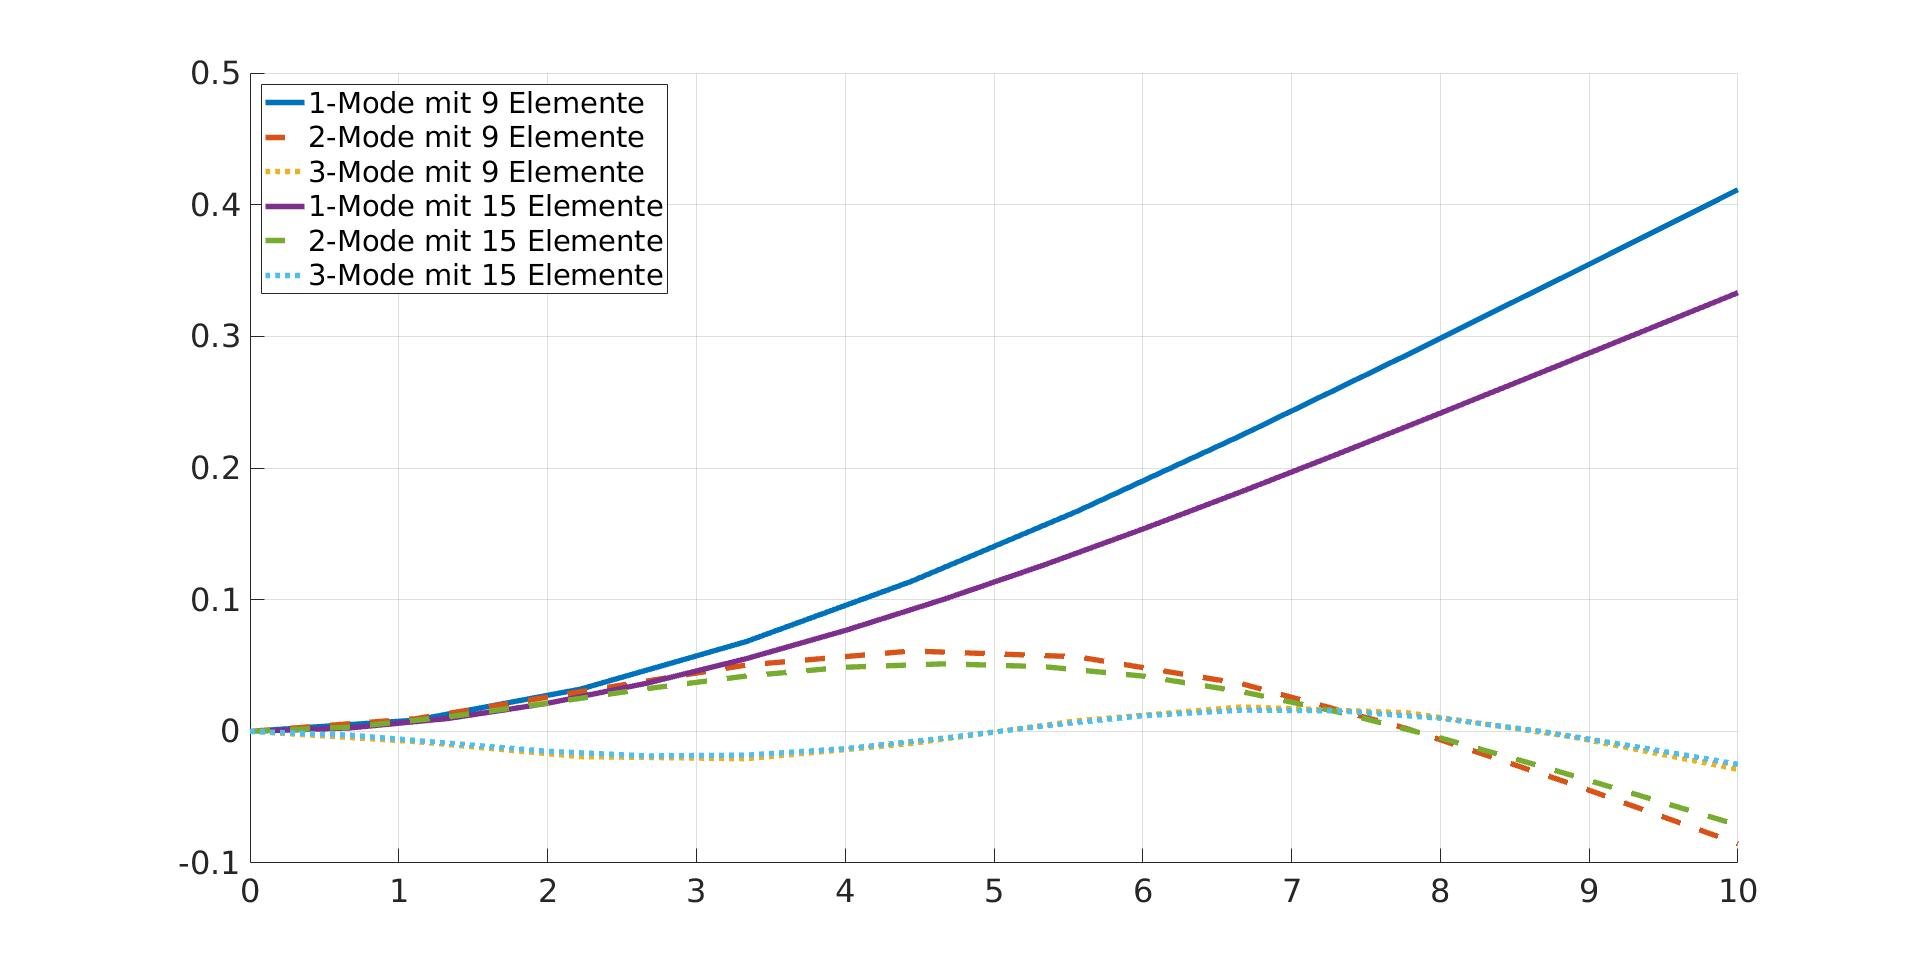
\includegraphics[width=1.0\linewidth, height=0.8\textheight]{Balken_9_15}
	\end{figure}
\end{frame}

\subsection{Biegeschwingungen einer Platte}
\begin{frame}{Biegeschwingungen einer Platte}
	\ \\
	Eigenfrequenzen
	\ \\
	\ \\
	\begin{table}[H]\label{tab:platten-RB}
		\renewcommand\arraystretch{1.3}
		\centering
		\resizebox{\textwidth}{11mm}{{\huge \textbf{		
			\begin{tabular}{|c|c|c|c|c|c|c|c|c|c|}
				\hline
				\diagbox[]{Eigenfrequenz [Hz]}{Mode}                              & 1        & 2        & 3         & 4         & 5         & 6         & 7         & 8         & 9         \\
				\hline
				9 Elemente je Seite & 2,162105 & 5,299083 & 13,259113 & 16,940469 & 19,284920 & 33,759497 & 38,167191 & 39,961917 & 44,225406 \\
				\hline	
				15 Elemente je Seite & 2,161776 & 5,298090 & 13,256507 & 16,938819 & 19,280190 & 33,748742 & 38,150961 & 39,947782 & 44,201679\\
				\hline	 
				Ergebnis \Ansys & 2,161505 & 5,293666 & 13,254572 & 16,932654 & 19,265101 & 33,713487 & 38,157460 & 39,942079 & 44,185442 \\
				\hline
		\end{tabular}}}}
	\end{table}
\end{frame}

\begin{frame}{Biegeschwingungen einer Platte}
	Eigenschwingformen
	\begin{figure}
		\centering
		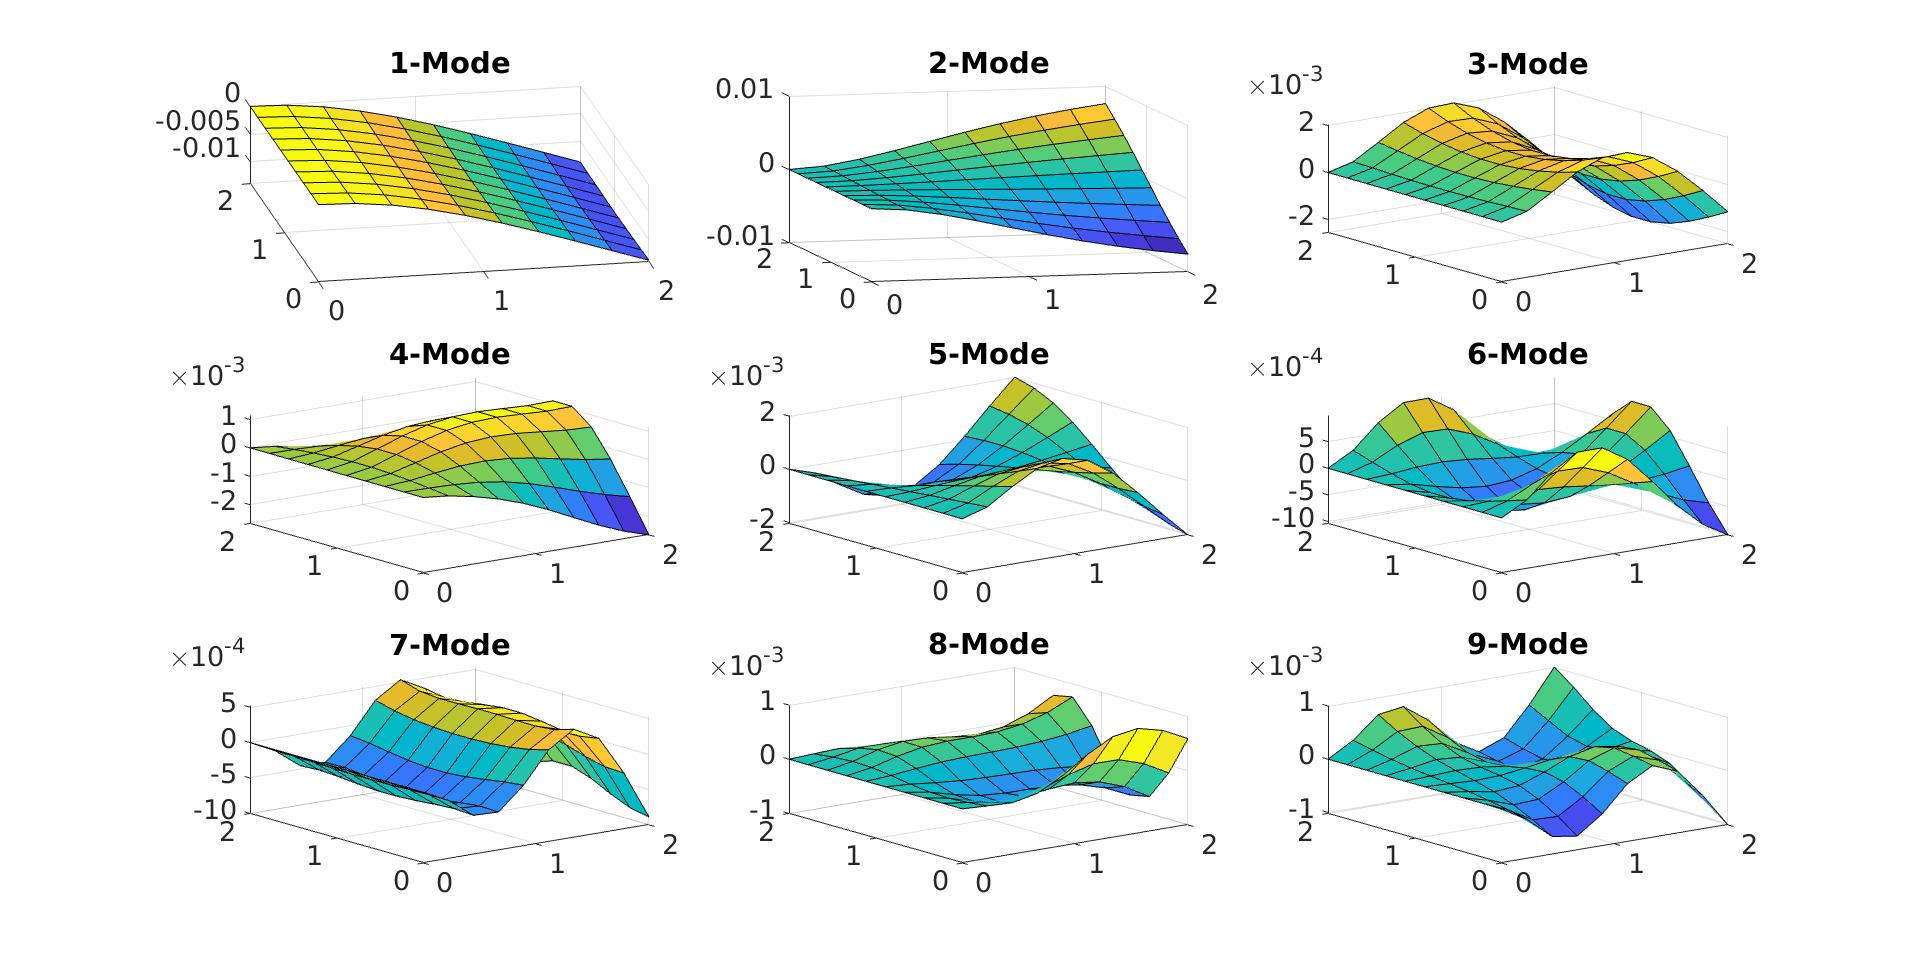
\includegraphics[width=1.0\linewidth, height=0.8\textheight]{Platten_RB_9}
	\end{figure}
\end{frame}

\begin{frame}{Biegeschwingungen einer Platte}
	Eigenschwingformen
	\begin{figure}
		\centering
		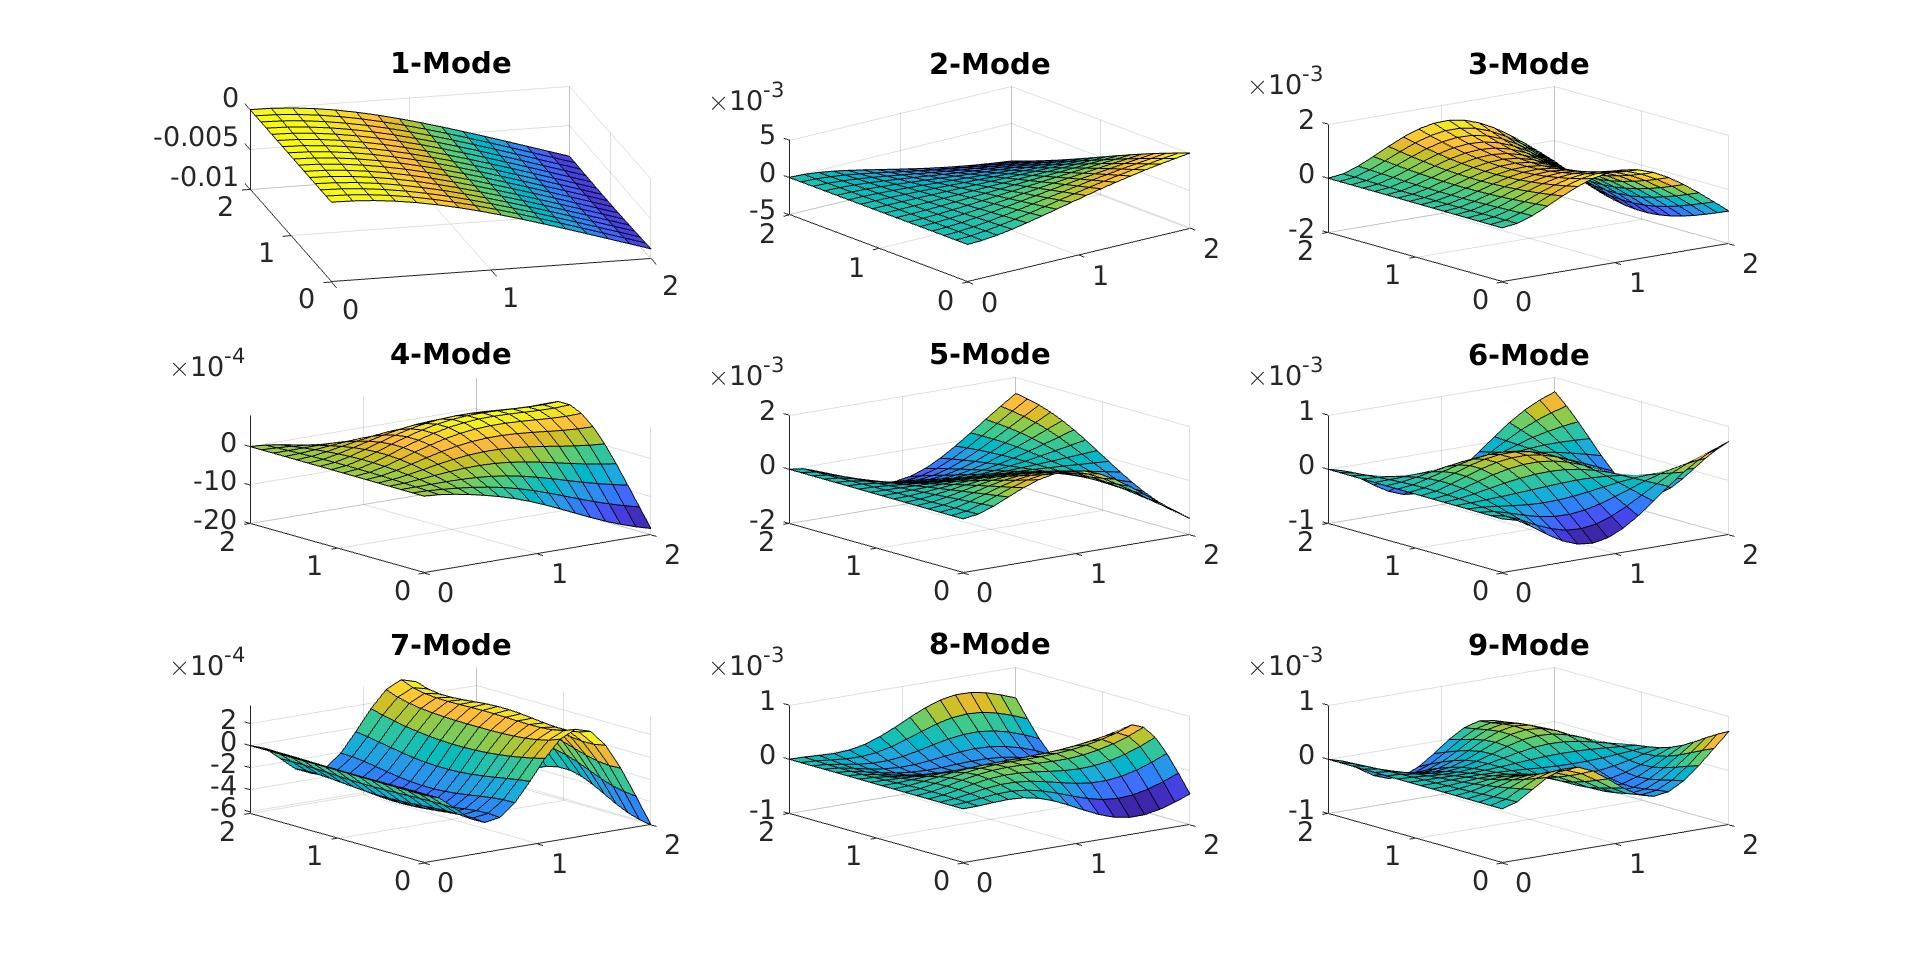
\includegraphics[width=1.0\linewidth, height=0.8\textheight]{Platten_RB_15}
	\end{figure}
\end{frame}




\section{Zusammenfassung/Ausblick}
\begin{frame}
	\begin{alertblock}{Zusammenfassung}
		Theoretische Grundlagen der numerischen Modalanalyse:\\
		\XBox Finite-Elemente-Methode\\
		\XBox Prinzip von Hamilton\\
		\ \\ 
		Durchgeführte Simulationen für folgende Beispiele:
		\XBox eindimensionales Modell (Stab)\\
		\XBox eindimensionales Modell (Balken)\\
		\XBox zweidimensionales Modell (Platte) \\	
	\end{alertblock}

	\pause
	
	\begin{TUBAFoutblock}{Ausblick}
		Modalanalyse für: \\ 
		\Square dreidimensionales Modell $ \Rightarrow $ nächster Schritt 
	\end{TUBAFoutblock}
\end{frame}

\section{ }
\begin{frame}[allowframebreaks]{Literatur}
	\nocite{*}
	\bibliography{Presentation}
\end{frame}

\begin{frame}{ \ }
{\LARGE 
	\ \\
	Vielen Dank für Ihre Aufmerksamkeit}
\end{frame}

%%%%%%%%%%%%%%%%%%%%%%%%%%%%%%%%%%%%%%%%%%%%%%%%%%%%%%%%%%%%%%%%%%%%%%%%%%%%%%%%%



\end{document}
